\documentclass[main.tex]{subfiles}

\begin{document}
\subsubsection{Project overview}
For the project, you will be submitting the following:
\begin{enumerate}
\item With Lab ~\ref{apx:lab_02}:
	\begin{enumerate}
	\item Photo Policy Acknowledgement
	\item Camera calibration grid photos
	\end{enumerate}
\item Project 1st part:
	\begin{enumerate}
	\item 1st sunset(/sunrise) photo
	\item Location documentation photo(s)/information
	\end{enumerate}
\item Project 2nd part:
	\begin{enumerate}
	\item 2nd sunset(/sunrise) photo
	\item 3rd sunset(/sunrise) photo
	\item Annotated photo
	\item Stellarium screenshots
	\item Project report
	\end{enumerate}
\end{enumerate}
\textbf{DO NOT WAIT TO TAKE YOUR PHOTOS!} The 3rd photo must be at least 4 weeks after the 1st, so if you leave the project to the last minute, you \textbf{will} lose points.

\subsubsection{Photo Policy Acknowledgement}
Make sure you read through the Photo Policy and submit your acknowledgement. Otherwise, you will not get credit for any of your submissions.

\textbf{Submitting work or pictures that are not your own, or having someone else do it for you, is a violation of academic integrity and will be dealt with harshly.}

\subsubsection{Camera calibration grid photos}
As part of Lab ~\ref{apx:lab_02}, submit photos of the zoomed-in and zoomed-out calibration grids.

The purpose of the activity is to help you work out the angular field of view of your camera, which you will make use of in the project. Hence, it is important that you use the \textbf{same} camera for all the sunset(/sunrise) photos, and to do the calibration. If this is not possible, let us know \textbf{as soon as you can}.

\subsubsection{Sunset photos}
The goal of the project is to obtain 3 pictures of the sunset OR sunrise from the exact same location, spaced apart in time. It is important that all 3 photos are consistent, i.e. they must EITHER be of the sunset OR the sunrise, not a mix. If this is not possible, let us know \textbf{as soon as you can}.

When you take the picture, ensure that:
\begin{enumerate}
\item your camera is zoomed out to zoom factor 1 (if your camera has a wide-angle function that can zoom out to a value lower than 1, e.g. 0.7 or similar, \textbf{do not use it})
\item the Sun is within about \SI{5}{\degree} in altitude of the horizon
\item the Sun's azimuth can be clearly discerned. Refer to the lecture during lab for examples of acceptable and unacceptable photos.
\end{enumerate}
Don't delete failed pictures! You can still get partial credit for attempts.

For the submission of the 1st part of the project, submit the 1st sunset(/sunrise) photo, along with documentation of the location you took it from.

For the other photos in the project, you must take them from the exact same location. The 2nd photo must be at least 1 week after the 1st photo, and the 3rd photo must be at least 4 weeks after the 1st photo AS WELL AS at least 1 week after the 2nd photo, as per Fig. ~\ref{fig:phottime}.
\begin{figure}[htb]
\begin{center}
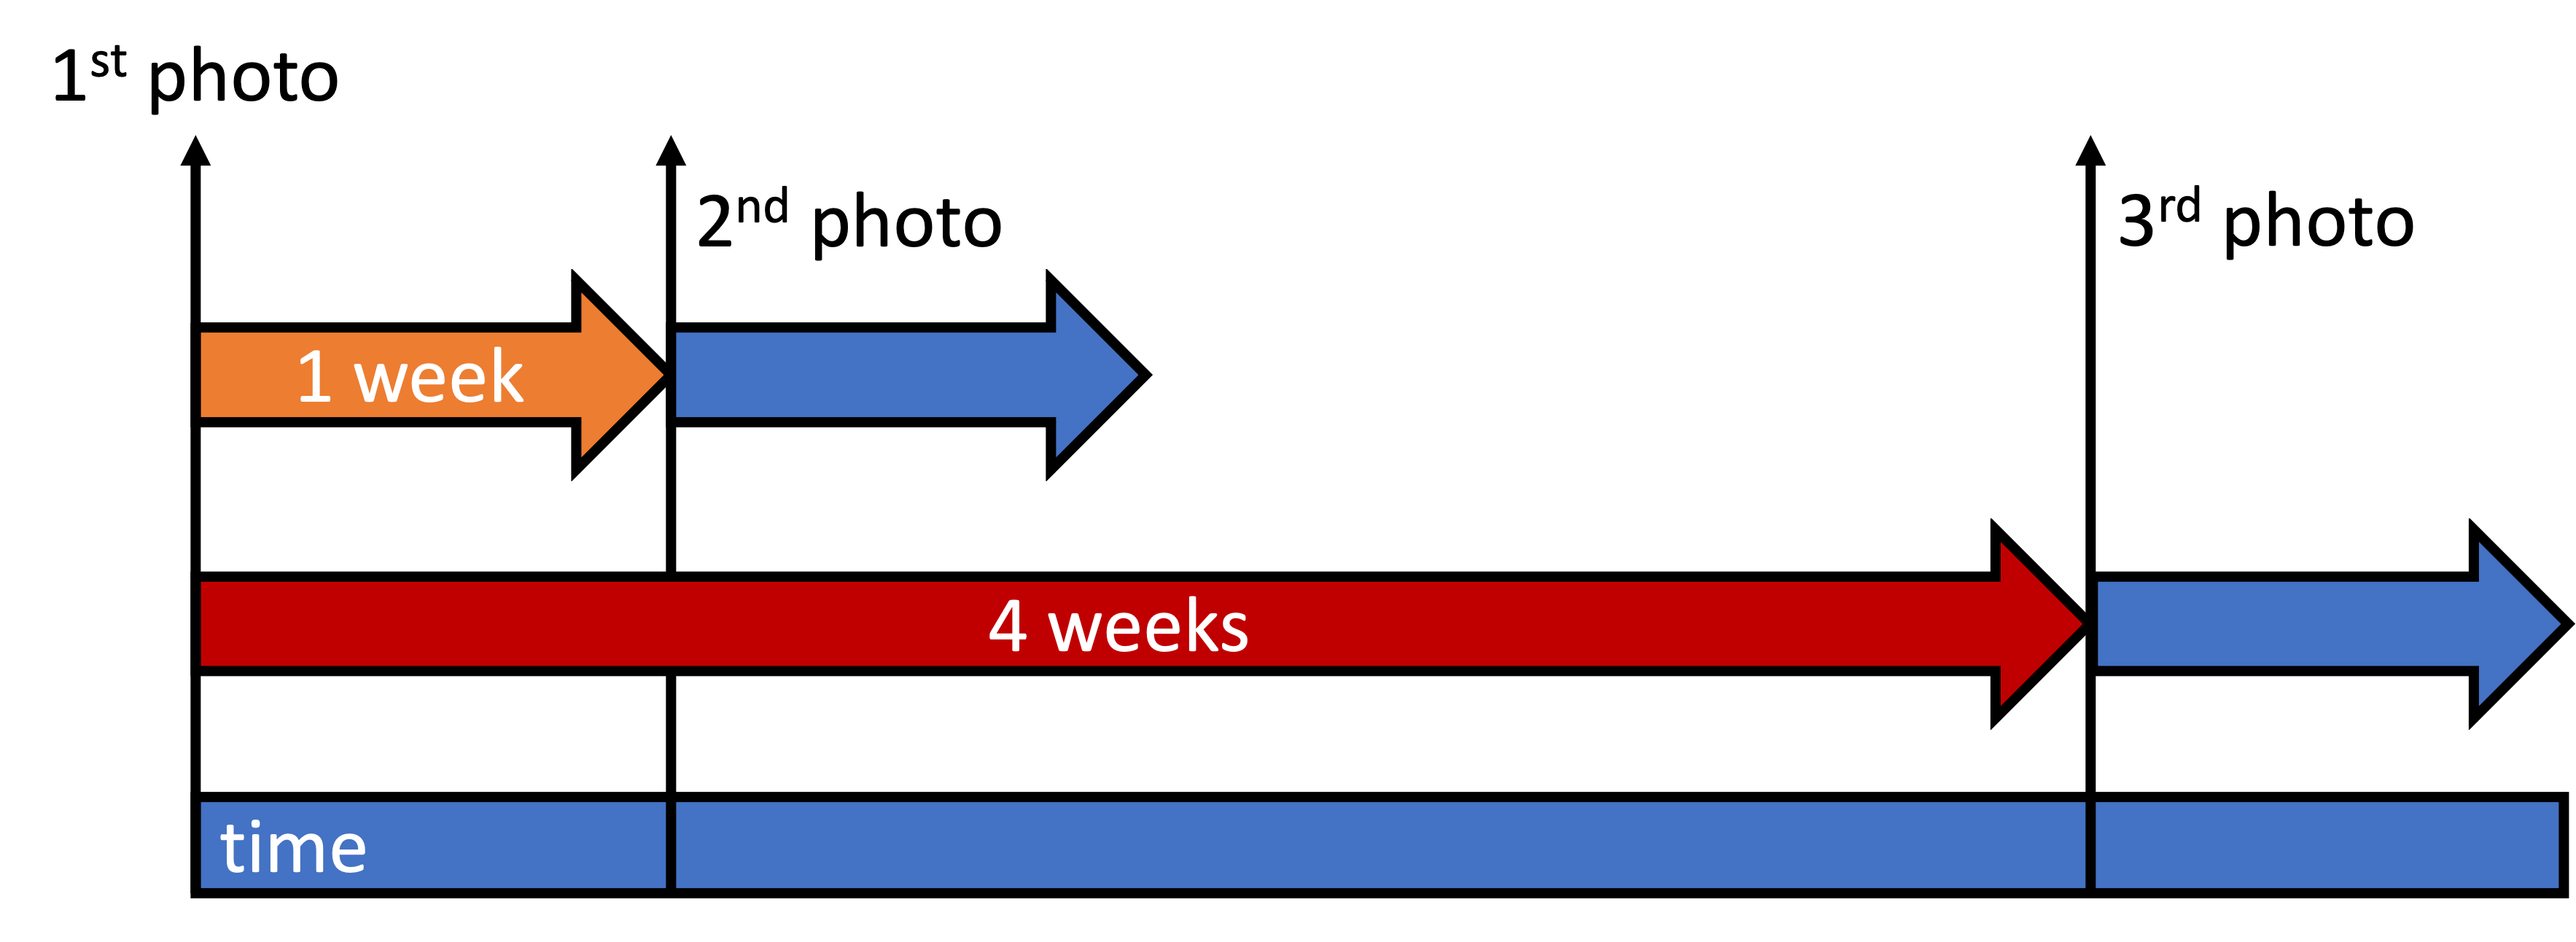
\includegraphics[width=0.6\textwidth]{photo_time.png}
\caption{Diagram of time spacing for sunset(/sunrise) photos.}
\label{fig:phottime}
\end{center}
\end{figure}

Submit the 2nd and 3rd photos as part of the 2nd part of the project.

\subsubsection{Location documentation}
All 3 photos must be taken from the same location. Bearing this in mind, we advise you to pick a location where:
\begin{enumerate}
\item you can get to the location again regularly later in the semester
\item a clear view of the horizon is visible
\item an area of the horizon is visible along which the sunset(/sunrise) will shift along over time.

In the spring, the sunset shifts north over time, which is to the right, and vice versa for the sunrise. This is reversed in the autumn.
\item there are features on the horizon that allow you to pinpoint the exact position of the sunset and how it moves over time. Refer to the lecture during lab for examples of acceptable and unacceptable photos.
\end{enumerate}

Additionally, it is important that you precisely document your location. You should provide enough information such that others can return to it and replicate your pictures. You will probably need to include a map along with photos that show clearly where you are standing when you take the pictures. Similar to the sunset photos, make sure features around your location are visible so your precise location can be pinpointed.

Submit the location documentation along with the 1st sunset photo for the 1st part of the project.

\subsubsection{Stellarium screenshots}
As we have in other labs, you'll set Stellarium to show the view from the same location and time as your photos, and then take screenshots, which you will submit. You can also click on the Sun to display information about it, including its altitude and azimuth, which we will ask you to report in the project report. These are meant to help you double-check your answers and help you get points.

Submit 1 screenshot corresponding to each of the 3 photos for the 2nd part of the project.

\subsubsection{Annotated photo}
The annotated photo is a \textbf{copy} of one of your photos, on which you will mark the positions of the sunsets from your other photos. Also, based on the angular scale of your camera (from calibrating it in Lab ~\ref{apx:lab_02}), predict where the sunset will shift to on 21 Dec (for fall semester)/21 Jun (for spring semester) and mark this position as well. You can make use of your calibration grid pictures for this. Fig. ~\ref{fig:photanot} shows a diagram of how the photo might look.
\begin{figure}[htb]
\begin{center}
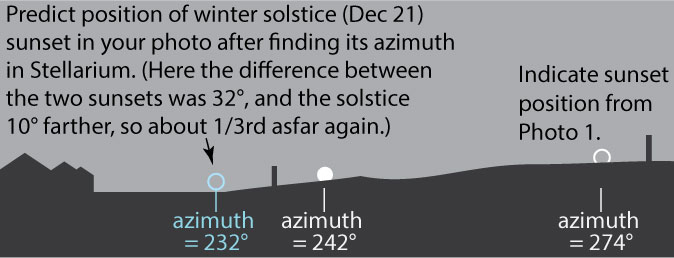
\includegraphics[width=0.5\textwidth]{sunset-pictures-fall-diagram.jpg}
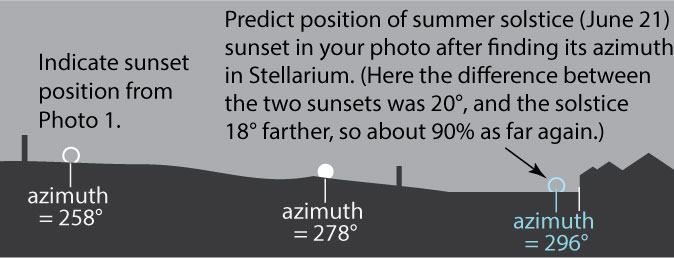
\includegraphics[width=0.5\textwidth]{sunset-pictures-spring-diagram.jpg}
\caption{}
\label{fig:photanot}
\end{center}
\end{figure}

Submit the annotated photo as part of the write-up of the project report, which is part of the 2nd part of the project.

\subsubsection{Project report}
The project report consists of a quiz section and write-up section, both on Moodle. You will not have a submit a separate document for it.

The quiz section will have you enter specifics about your photos, including date, time, azimuth of sunset, calibrated angular field of view, and so on. The write-up section will ask you to explain the procedure you used for predicting the position of the sunset(/sunrise) on the 21 Dec (for fall semester)/21 Jun (for spring semester) and locating it in the horizon view in your photo.

Note that the annotated photo is part of the submission for the write-up section. This does not, however, mean that either can be substituted for the other, i.e. an annotated photo cannot be taken to replace the write-up, or vice versa.

Happy touching grass!

\end{document}